\documentclass[8pt]{beamer}

\setbeamertemplate{background canvas}[vertical shading][bottom=cyan!10,top=blue!10]

\usetheme{metropolis}
\usefonttheme[onlysmall]{structurebold}

% pour le fichiers .pdf
\usepackage{graphicx}
\usepackage{color}
% pour les fichiers .png
% \usepackage{pgf,pgfarrows}
% \usepackage{pgf,pgfarrows}
\usepackage{amsmath,amssymb}
\usepackage{textcomp}
\usepackage{multitoc}
\usepackage{mdwtab}
\usepackage{hyperref}
\setbeamercovered{dynamic}
\DeclareMathOperator*{\argmin}{argmin}

\hypersetup{
    bookmarks=true,         % show bookmarks bar?
    unicode=false,          % non-Latin characters in Acrobat's bookmarks
    pdftoolbar=true,        % show Acrobat's toolbar?
    pdfmenubar=true,        % show Acrobat's menu?
    pdffitwindow=false,     % window fit to page when opened
    pdfstartview={FitH},    % fits the width of the page to the window
    pdftitle={Tutorial OpenTURNS},    % title
    pdfauthor={HADDAD},     % author
    pdfsubject={Starting with OpenTURNS},   % subject of the document
    pdfproducer={Producer}, % producer of the document
    pdfkeywords={keyword1} {key2} {key3}, % list of keywords
    pdfnewwindow=true,      % links in new window
    colorlinks=true,       % false: boxed links; true: colored links
    linkcolor=red,          % color of internal links
    citecolor=green,        % color of links to bibliography
    filecolor=magenta,      % color of file links
    urlcolor=blue          % color of external links
}

\title[OpenTURNS modules development]{OpenTURNS modules development}
\author[OpenTURNS Consortium, 2022]
{
  Trainer : Sofiane Haddad\\
  Airbus \\
  sofiane.s.haddad@airbus.com
}



\date[Fab 14-17th 2022]
{
  Developers training \\

  \begin{center}
    \includegraphics[height=2cm]{figures/logoOT.jpg}
  \end{center}
}

\subject{OpenTURNS Developers Training}

% \part<presentation>{Corps de presentation}


\begin{document}

\frame{\titlepage}

% necessaire pour la table des matieres
\part{Main part}

% table des matieres
\begin{frame}
  \frametitle{OpenTURNS modules development}
  \tableofcontents[part=1]
\end{frame}
%%%%%%%%%%%%%%%%%%%%%%%%% 
% The OpenTURNS package %
%%%%%%%%%%%%%%%%%%%%%%%%% 
\section[OpenTURNS modules]{OpenTURNS modules}
%%%%%%%%%%%%% 
% The tools %
%%%%%%%%%%%%% 
\begin{frame}
  \frametitle{OpenTURNS modules: objectives}
  \begin{block}{}
    OpenTURNS is a growing system developed by a small team. A constant problem is to assess the stability of the whole product, and in order to achieve this goal we introduced a notion of module, in order to insulate a core library dedicated to the definition of the abstract data model and to propose all the specific algorithms as optional modules. The core would evolve quite slowly, insuring its robustness, whereas the modules would have a more dynamic development model.\\
    Another key objective is to provide a way to extend the existing platform with functionalities developed by teams that are reluctant to adopt the OpenTURNS development process. Within the module, the development team can adopt any coding rule or programming language he want, as long as the OpenTURNS interface is respected as well as the objects lifecycle.
  \end{block}
\end{frame}


\begin{frame}[containsverbatim]
  \frametitle{Current modules - a non exhaustive list}
  
  \alert{Modules} connected to the library and maintained by the consortium :
  \begin{itemize}
  \item \alert{otagrum} : create a distribution from a Bayesian Network using aGrUM
  \item \alert{otfftw} : Fast Fourier Transform algorithm (e.g. for stochastic processes) using FFTW
  \item \alert{otfmi} : FMI models manipulation using PyFMI
  \item \alert{otmixmod} : build mixtures of a multivariate Normal distribution from a sample
  \item \alert{otmorris} : Morris screening method module
  \item \alert{otpmml} : manages PMML files for meta-modeling exchanges
  \item \alert{otpod}: A module to build Probability of Detection for Non Destructive Testing
  \item \alert{otrobopt}: robust optimization
  \item \alert{otsubsetinverse}: inverse subset simulation
  \item \alert{otsvm} : Support Vector regression and classification with libsvm
  \item \alert{otwrapy} : Python wrapper tools
  \item \alert{otsklearn} : use OT surrogate models with the scikit-learn estimator API
  \end{itemize}
  
  Oldest modules:
  \begin{itemize}
  \item \alert{otlm} Linear model with stepwise strategies
  \item \alert{otlhs} Optimal LHS (Monte-Carlo \& Annealing)
  \item $\cdots$
  \end{itemize}
  \end{frame}
  
  \begin{frame}[containsverbatim]
    \frametitle{Current modules - a non exhaustive list}
    
    \alert{Other modules} connected to the library :
    \begin{itemize}
    \item \alert{otbenchmark} : benchmark problems for reliability and sensitivity analysis
    \item \alert{othdrplot}: high density region algorithm for functional outlier detection
    \item \alert{otsurrogate}: surrogate models
    \item \alert{otusecases}: use cases suitable for OpenTURNS (functions and datasets)
    \item \alert{otmarkov}: simulates Markov chains (experimental)
    \item \alert{otsensitivity} : sensitivity analysis with density based measures
    \item \alert{shapley-effects} : compute Shapley effects
    \item \alert{batman} : Statistical analysis for expensive computer codes made easy.
    \item \alert{otpod} : Probability of Detection module.
    \item \alert{otgu} : Gu method to make more robust the estimation kriging models.
    \item \alert{others} : need to reactivate some oldest modules (\texttt{otgmm}, \texttt{pygosa}, \texttt{otfitting}, \texttt{othsic}) and others
  \end{itemize}
    \end{frame}
    
  
\begin{frame}
  \frametitle{OpenTURNS modules - C++}
  \centering \resizebox{!}{4cm}{\includegraphics{figures/OTModule.pdf}}
  \begin{block}{The principles}
    An OpenTURNS module is typically made of two parts:
    \begin{itemize}
    \item a C++ part that uses the OpenTURNS C++ interface in order to provide new specialization or to produce instances of the data model using new algorithms with no OpenTURNS counterpart.
    \item a Python part, the Python interface of the C++ part, often obtained using SWIG. In this case, this SWIG interface must use the OpenTURNS interface the same way its C++ interface uses the OpenTURNS C++ interface.
    \end{itemize}
  \end{block}
\end{frame}

\section[Module development]{Module development - C++}
\begin{frame}
  \frametitle{Module development}
  \begin{block}{Step 1: copy and adapt an existing template}
    \begin{itemize}
    \item Copy and rename the source tree of an example module (for example the Strange module) from the OpenTURNS source tree. The examples modules are located under the module subdirectory of OpenTURNS source tree:\\
      {\ttfamily git clone https://github.com/openturns/ottemplate.git MyModule template }
    \item Set the url of the remote (meaning you already created a repository):\\
      {\ttfamily git remote set-url origin https://github.com/USERNAME/REPOSITORY.git}
    \item Adapt the template to your module:\\
      {\ttfamily ./customize.sh MyModule MyModuleClass}\\
      This command change the module name into all the scripts, and adapt the example class to this new name.
    \end{itemize}
  \end{block}
\end{frame}

\begin{frame}
  \frametitle{Module development}
  \begin{block}{Step 2: develop the module}
    \begin{itemize}
    \item Implement your module. You are free to use the rules you want, but if the final objective of the module is to be integrated in the official release of OpenTURNS, it is wise to adopt the OpenTURNS development process and rules.
    \item Build your module as usual:
      \begin{tabular}{l}
        \ttfamily mkdir build\\
        \ttfamily cd build\\
        \ttfamily cmake .. -DCMAKE\_INSTALL\_PREFIX=INSTALLDIR \\
        \ttfamily -DOpenTURNS\_DIR=OPENTURNS\_INSTALLDIR/lib/cmake/openturns\\
        \ttfamily make
      \end{tabular}
    \item Create a source package of your module:\\
      {\ttfamily make package\_source}\\
      It will create a tarball named mymodule-X.Y.Z.tar.gz (and mymodule-X.Y.Z.tar.bz2), where X.Y.Z is the version number of the module.
    \end{itemize}
  \end{block}
\end{frame}


\begin{frame}
  \frametitle{Module development}
  \begin{block}{Step 3: documentation}
    Module documentation is very close to the API one:
    \begin{itemize}
    \item Developer guide : Architecture, validation
    \item SWIG documentation is to be completed (docstrings); 
    \item Examples and API documentation;
    \item Theory (if needed)
    \end{itemize}
  \end{block}
\end{frame}


\begin{frame}
  \frametitle{Module development}
  \begin{block}{Step 4: install and test the module}
    \begin{itemize}
    \item Check that you have a working OpenTURNS installation, for example by trying to load the OpenTURNS module within an interactive python session:
      \begin{tabular}{l}
        \ttfamily \$python\\
        \ttfamily >>> import openturns as ot\\
      and python should not complain about a non existing openturns module.\\
      \end{tabular}
    \item Since first step is ok, test your module within python:\\
      \begin{tabular}{l}
        \ttfamily \$python \\
        \ttfamily >>> import openturns as ot \\
        \ttfamily >>> import mymodule \\
      and python should not complain about a non existing mymodule module.
      \end{tabular}
      \item You can now use your module as any python module.
    \end{itemize}
  \end{block}
\end{frame}


\begin{frame}
  \frametitle{Module development}
  \begin{block}{Step 5: Maintenance}
    Each developer is responsible of his package should maintain it!
    \begin{itemize}
    \item We can rely on continuous integration tool accounting API changes
    \item He is in charge of bugs (except if underlying bug is in the API)
    \end{itemize}
    Exception : modules maintained by the consortium!
  \end{block}
  
  \begin{block}{Step 6: Packaging}
    No specific rule concerning the packaging!
    \begin{itemize}
    \item Tarball generation
    \item Git
    \item conda...
    \end{itemize}
    Exception : modules maintained by the consortium!
  \end{block}
\end{frame}


\section[Module development]{Module development - Pure python module}
  \begin{frame}[containsverbatim]
    \frametitle{And for a Python module?}
        
    Python eco-system:
    \begin{itemize}
    \item \alert{numpy/scipy} : scientific usage 
    \item \alert{scikit-learn} : Machine-Learning algorithms
    \item \alert{pydoe, pydoe2} : Design of experiment
    \item \alert{chaospy} : Polynomial chaos expansion
    \item \alert{pandas} : Data analysis
    \item \alert{SALib} : Sensitivity analysis library
    \item \alert{pymc3} : Fit bayesian models
    \item \alert{GPFlow, GPyTorch, TensorFlow, PyTorch, georges...  }
    \item \alert{statsmodels} : Statistical tools
    \item $\cdots$ many many 
    \end{itemize}
    \end{frame}



\begin{frame}
  \frametitle{Can my module be used by openturns algorithms?}
  \begin{block}{}
    For now, there is (almost) no way to use a Python object within the \texttt{OpenTURNS} C++ library, excepting:
    \begin{itemize}
    \item A Distribution;
    \item a Function;
    \item An experiment
    \item A RandomVector
    \item A FieldFunction
    \item $\hdots$
    \end{itemize}
    and use these one as "OpenTURNS classes".\\

    The concept of "OpenTURNS Python module" is not very specific: 
    we get some `full python` packages such as \texttt{oticp}, \texttt{otwrap} , \texttt{otsklearn}. 
    But these examples are in a way independent as they rely on the "OpenTURNS API" and the API is not able to `integrate` them.
    For example :
    \begin{itemize}
    \item Optimization toolbox even if it relies on \texttt{openturns} objects;
    \item Surrogate models - Could not inherit from \texttt{MetaModelAlgorithm} 
    \item kernels - Could not inherit from \texttt{CovarianceModel} 
    \item $\hdots$
    \end{itemize}
    But many often, the objective is to \texttt{build openturns classes} such as \texttt{Experiment, Function}!
    
    In other words, any set of Python classes or Python functions that use the OpenTURNS Python interface can be called an OpenTURNS Python module. 
    In this case, the notion of OpenTURNS module is mainly a packaging notion, and the use of the Python setup tools is probably more mature and more adapted!
  \end{block}
\end{frame}

\begin{frame}
  \frametitle{No existing (official) template}
  \begin{block}{}
    In comparison with C++, there is no template: 
    \begin{itemize}
    \item Such a module might be some development using \texttt{openturns} classes or not;
    \item Such a development relies on external modules (\texttt{scikit-learn, rpy2} for example) 
    \item Such a development makes others benefit from \texttt{openturns} in a friendly framework (\texttt{scikit-learn} for example)
    \item $\hdots$
    \end{itemize}
    Why ?
    \begin{itemize}
      \item Such a development relies on external modules (\texttt{scikit-learn, rpy2} for example) 
      \item Such a development makes others benefit from \texttt{openturns} in a friendly framework (\texttt{scikit-learn} for example)
      \end{itemize}
      Non-official templates:
      \begin{itemize}
        \item \href{https://github.com/adumasphi/ottemplatepython}{Template done by Antoine Dumas}
        \item \href{https://github.com/sofianehaddad/ottemplatepython.git}{new template}
        \end{itemize}
  \end{block}
\end{frame}

\begin{frame}
  \frametitle{How to proceed?}
  \begin{block}{Identify the needs}     
    \begin{itemize}
      \item Why do we need an Openturns interface? 
      \item Do I need to link to an external module? If yes what kind of data or objects is required?
      \item What does my module require and provide? 
      \item What kind of interaction with the API?
    \end{itemize}
  \end{block}
\end{frame}

\begin{frame}
  \frametitle{Module development}
  \begin{block}{Step 1: copy and adapt an existing template (even if non official) or start from crash}
    \begin{itemize}
    \item Copy and rename the source tree of an example module (for example the Strange module) from the OpenTURNS source tree. The examples modules are located under the module subdirectory of OpenTURNS source tree:\\
      {\ttfamily git clone \href{https://github.com/sofianehaddad/ottemplatepython.git}{https://github.com/sofianehaddad/ottemplatepython.git} MyModule}
    \item Set the url of the remote (meaning you already created a repository):\\
      {\ttfamily git remote set-url origin https://github.com/USERNAME/REPOSITORY.git}
    \item Adapt the template to your module:\\
      {\ttfamily no customize.sh }\\
      Rename folder to the new module, update tests and doc.
    \end{itemize}
  \end{block}
\end{frame}

\begin{frame}
  \frametitle{Module development}
  \begin{block}{Step 2: develop the module}
    \begin{itemize}
    \item Implement your module. You are free to use the rules you want!
    \item Build \& install your module as usual:
      \begin{tabular}{l}
        \ttfamily python setup.py build \\
        \ttfamily python setup.py install
      \end{tabular}
    \end{itemize}
  \end{block}
\end{frame}


\begin{frame}
  \frametitle{Module development}
  \begin{block}{Step 3: documentation}
    Module documentation is very "easy". 
    \begin{itemize}
      \item Document classes and method using python peps
      \item Developer guide : Architecture, validation
      \item Examples and API documentation (potentially notebooks)
      \item Theory (if needed)
      \item Build the doc:
      \begin{tabular}{l}
        \ttfamily python setup.py build\_sphinx
      \end{tabular}
    \end{itemize}
  \end{block}
\end{frame}


\begin{frame}
  \frametitle{Module development}
  \begin{block}{Step 4: install and test the module}
    \begin{itemize}
    \item Since first step is ok, test your module within python:\\
      \begin{tabular}{l}
        \ttfamily \$python \\
        \ttfamily >>> import openturns as ot \\
        \ttfamily >>> import mymodule \\
      and python should not complain about a non existing mymodule module.
      \end{tabular}
      \item You can now use your module as any python module.
      \item For the setup, use \texttt{setuptools, distutils} 
      \item For the tests, rely on \texttt{openturns test}, \texttt{pytest} 
    \end{itemize}
  \end{block}
\end{frame}


\begin{frame}
  \frametitle{Module development}
  \begin{block}{Step 5: Maintenance}
    Each developer is responsible of his package should maintain it!
    \begin{itemize}
    \item We can rely on continuous integration tool accounting API changes
    \item He is in charge of bugs (except if underlying bug is in the API)
    \end{itemize}
  \end{block}
  
  \begin{block}{Step 6: Packaging}
    No specific rule concerning the packaging!
    \begin{itemize}
    \item Tarball generation
    \item Git
    \item conda\slash pip ...
    \item \ttfamily python setup.py sdist --formats=gztar,zip
  
    \end{itemize}
    Exception : modules maintained by the consortium!
  \end{block}
\end{frame}

\begin{frame}
  \frametitle{Module development: conda deployement}
  \begin{block}{}
    User should generates a recipe in \href{https://github.com/conda-forge/staged-recipes}{staged-recipes}.
    \begin{itemize}
    \item Rely on existing template
    \item Fork the repository
    \item Have a look at the documentation
    \item Adapt to the module and propose pull-request
    \end{itemize}
    In case of pure python it is more simple! Have a look at \href{https://github.com/conda-forge/staged-recipes/pull/14533}{tensap} for example.\\
    Once it is done, module is integrated to \texttt{conda-forge}
  \end{block}
\end{frame}

\begin{frame}
  \frametitle{Module development: pip}
    We can rely on this \href{https://www.geeksforgeeks.org/how-to-publish-python-package-at-pypi-using-twine-module}{blog} to upload the module:
    \begin{itemize}
    \item \ttfamily{pip install twine} : install the module that help the upload 
    \item We suppose the package is organized in a well format (Readme, License, module)
     \item \ttfamily{python setup.py bdist\_wheel} to create a .dist
     \item \ttfamily{twine upload dist/*} to upload. You should have an account on \href{pypi.org}{pypi} and enter credential when asked.
    \end{itemize}
\end{frame}

\begin{frame}
  \frametitle{Module development: upload documentation using github and continuous integration}
    We suppose here that we use \href{https://github.com}{github} for the maintenance. The purpose here is to illustrate how to deply\slash upload documentation after a commit on the main branch.
    \begin{itemize}
      \item Goto the \texttt{Developer settings} in your github account (see \href{https://github.com/settings/apps}{here})
      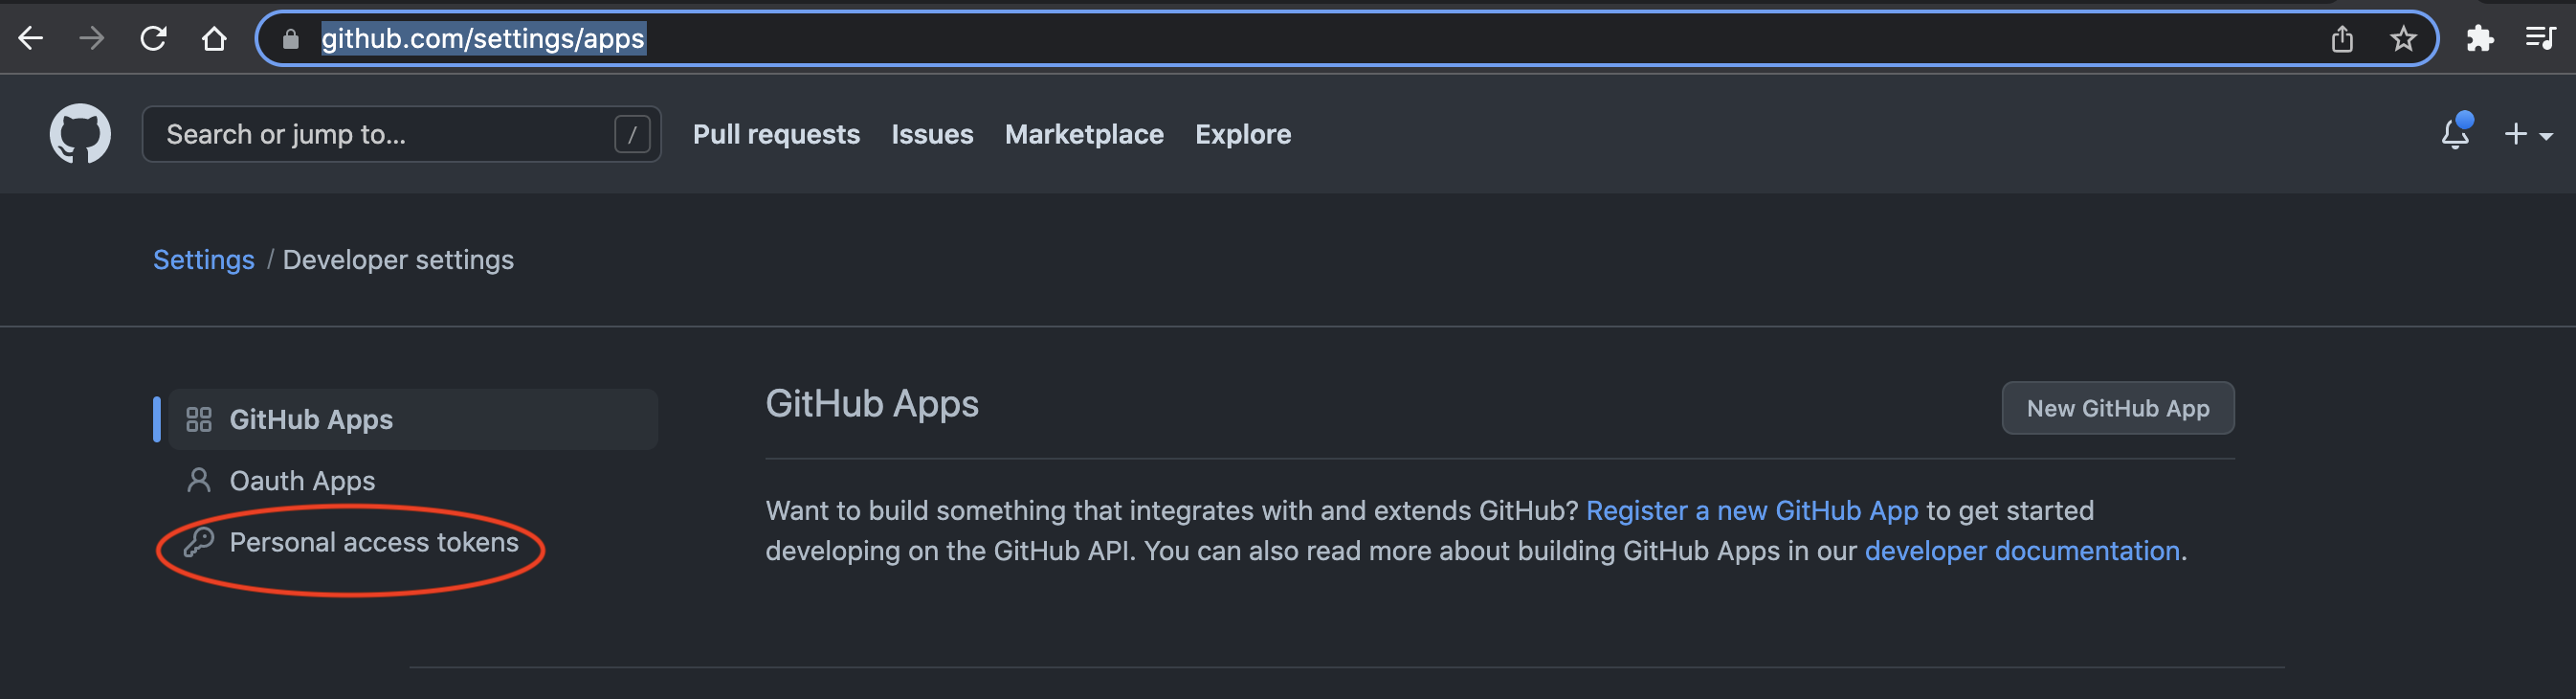
\includegraphics[width=10.cm]{github_settings.png}
      \item Select \texttt{Personal access tokens} and \texttt{Generate new token} \\
     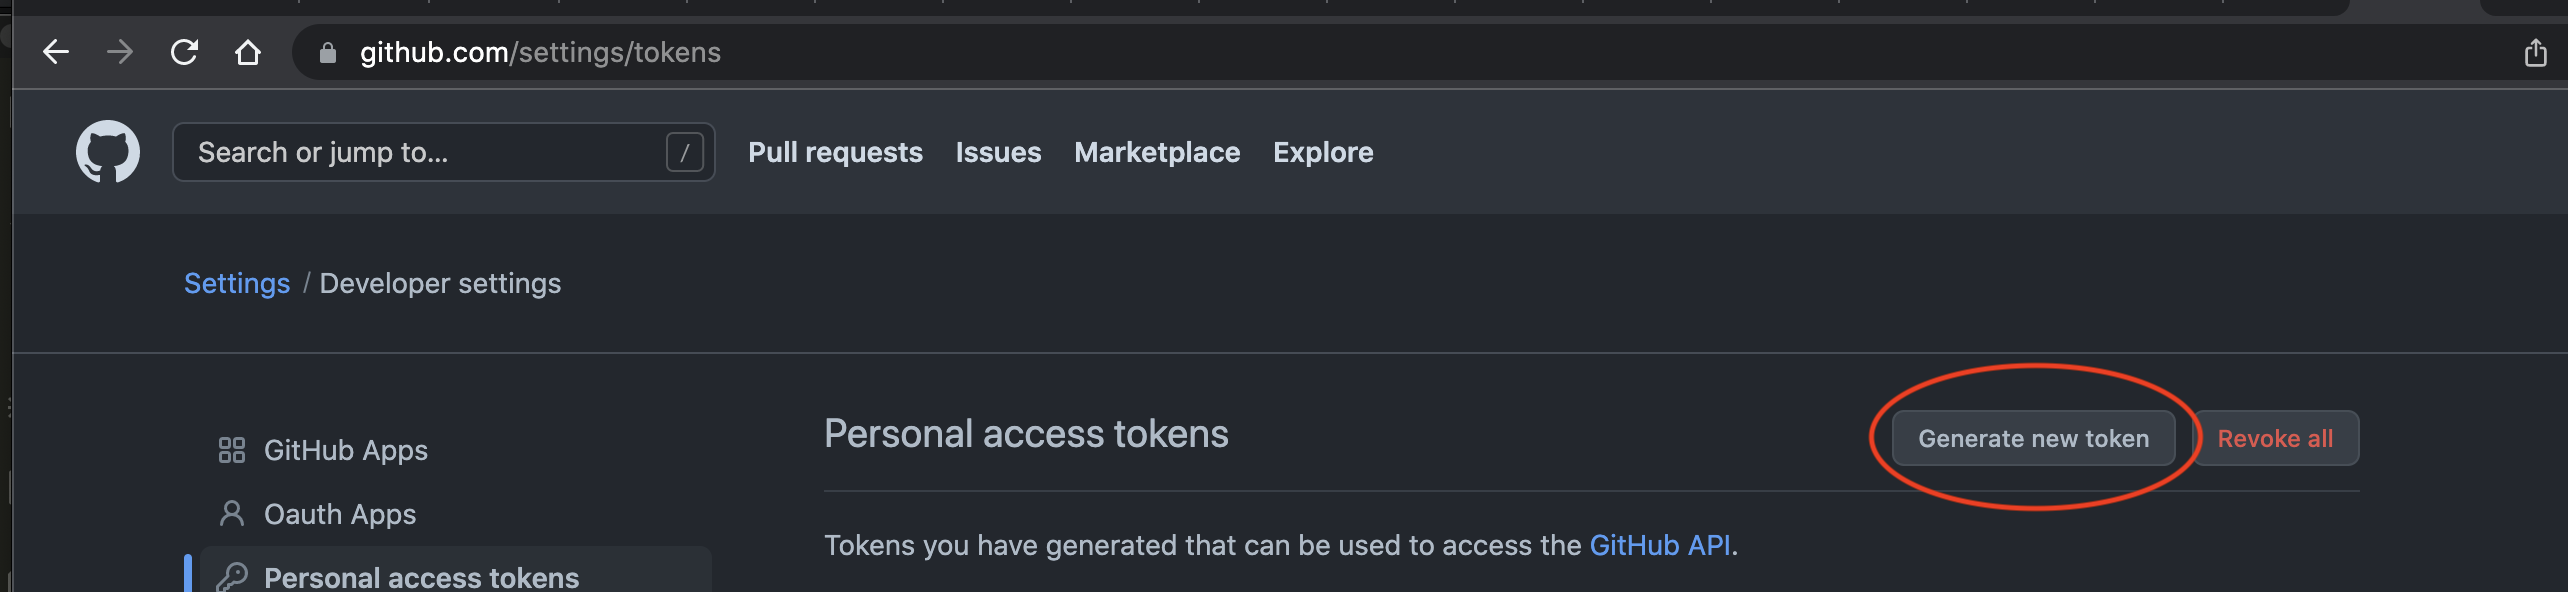
\includegraphics[width=8.cm]{generate_token.png}
    \end{itemize}
\end{frame}

\begin{frame}
  \frametitle{Module development: upload documentation using github and continuous integration}
    \begin{itemize}
      \item Provide a name (for example GH\_TOKEN) and select at least repo and workflow
     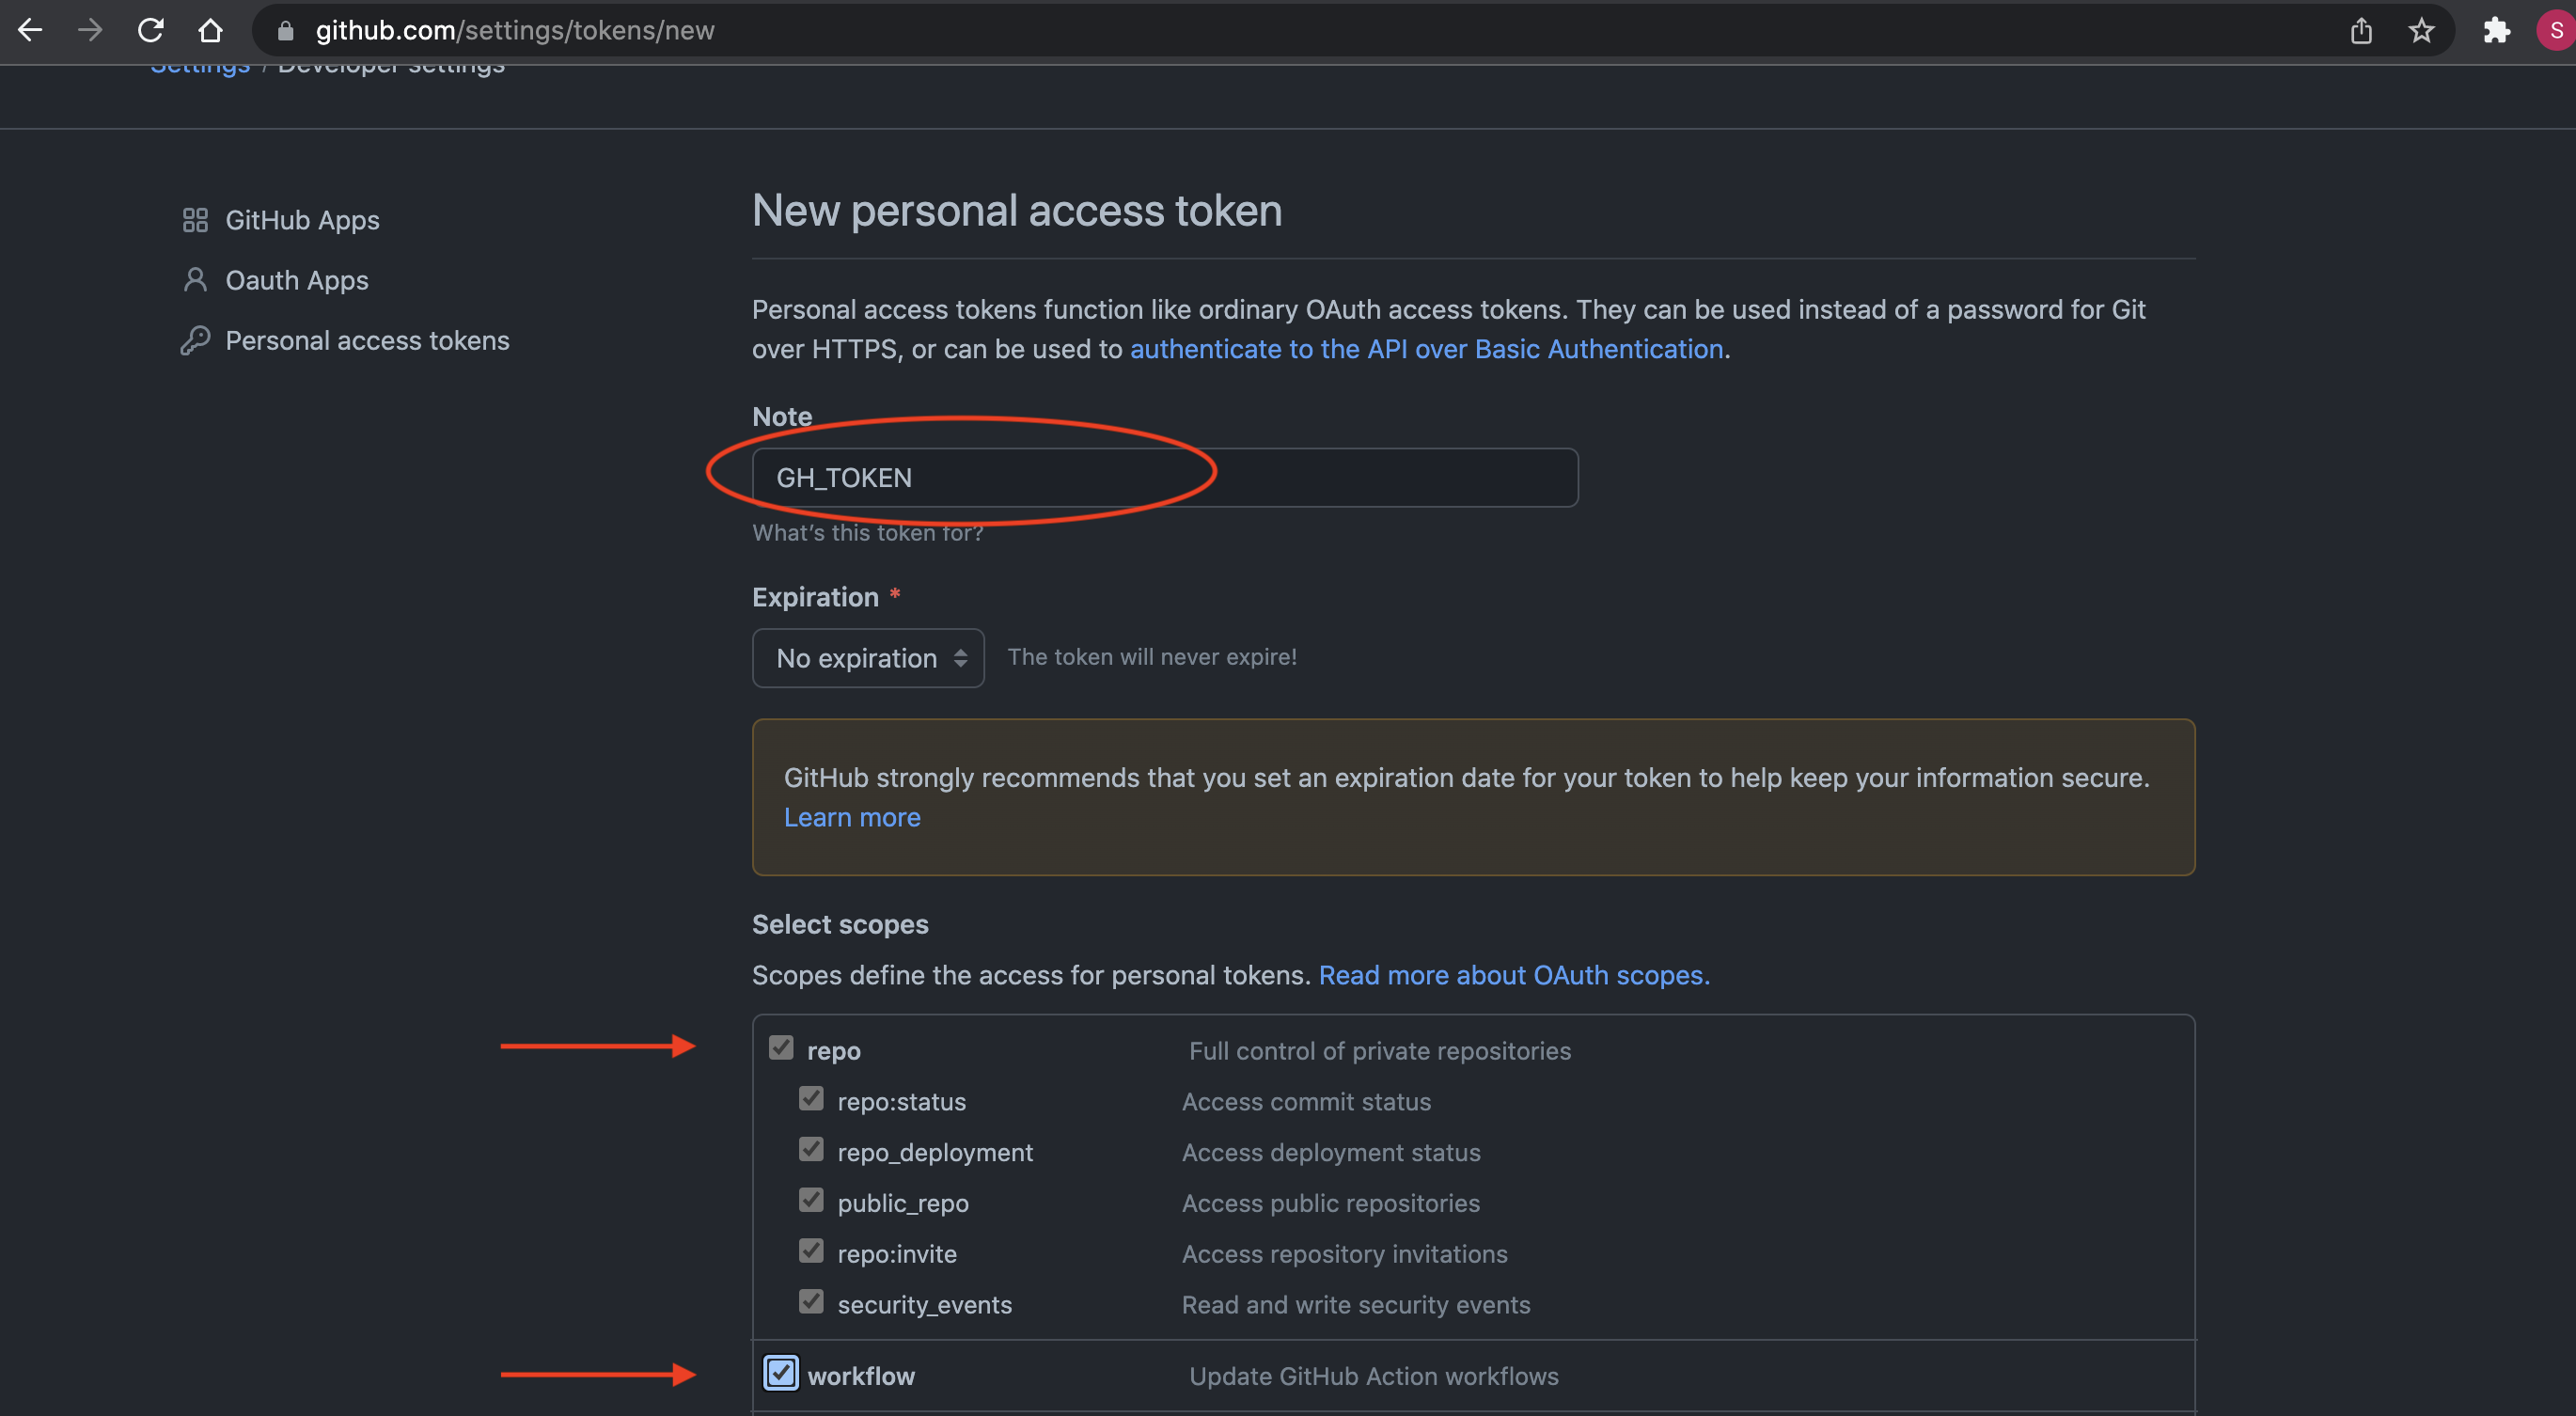
\includegraphics[width=8.cm, height=4cm]{new_token.png}
    \item At the end, we generate a token
    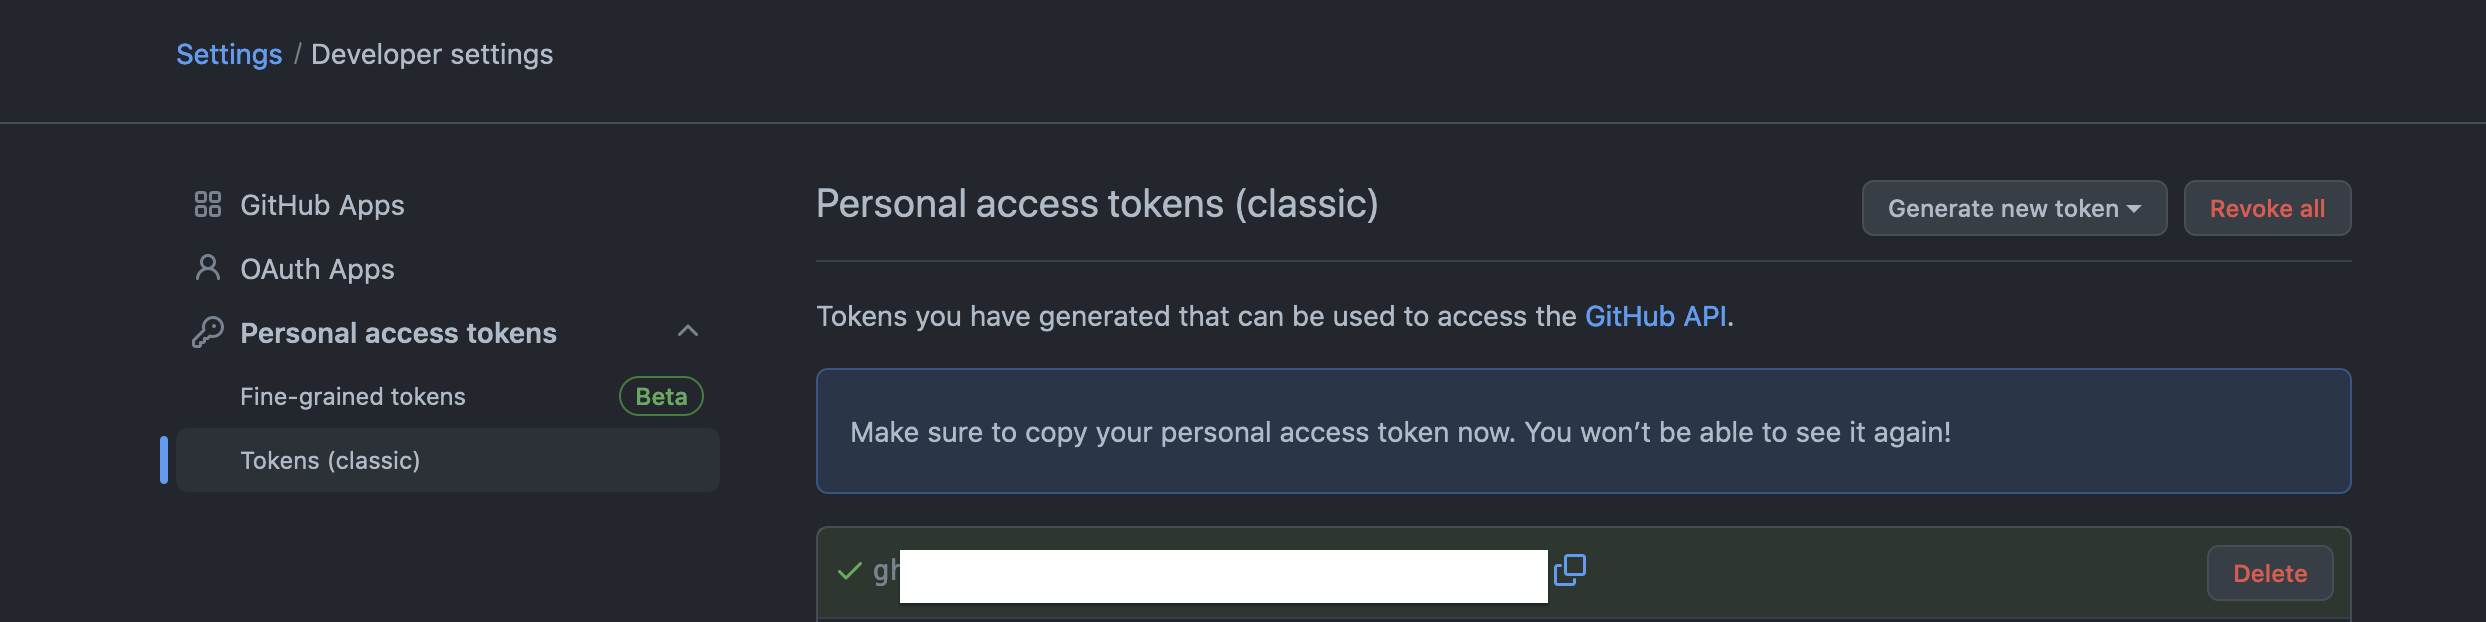
\includegraphics[width=8.cm, height=2cm]{generated_token.png}
    \item We should store\slash copy this token as it will be used later.
      \end{itemize}
\end{frame}

\begin{frame}
  \frametitle{Module development: upload documentation using github and continuous integration}
  Now we should feed corresponding project with the previous token. For that:

    \begin{itemize}
      \item On github, reach the settings corresponding to the repository of interest.
      \item On the left, select the \texttt{Secret} and \texttt{Actions}\\
      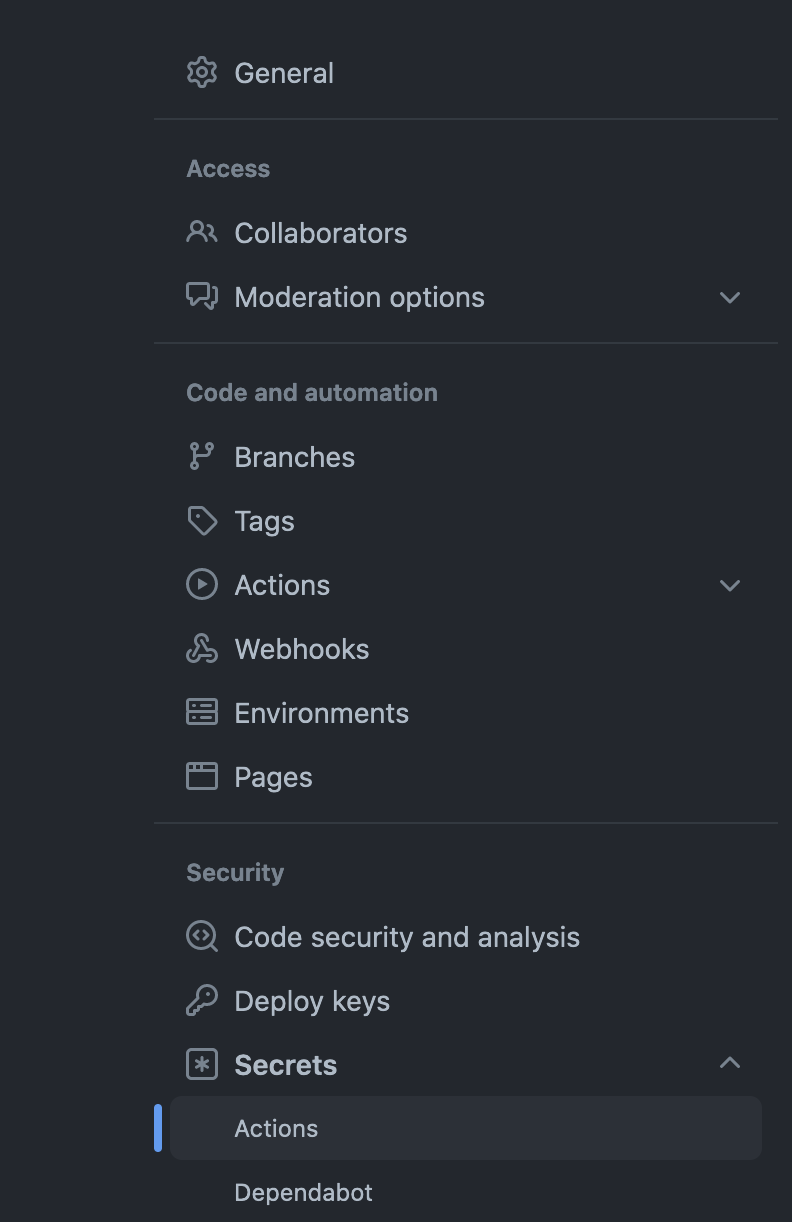
\includegraphics[width=2.cm, height=5cm]{select_action.png}
      \item Generate new repository secret
      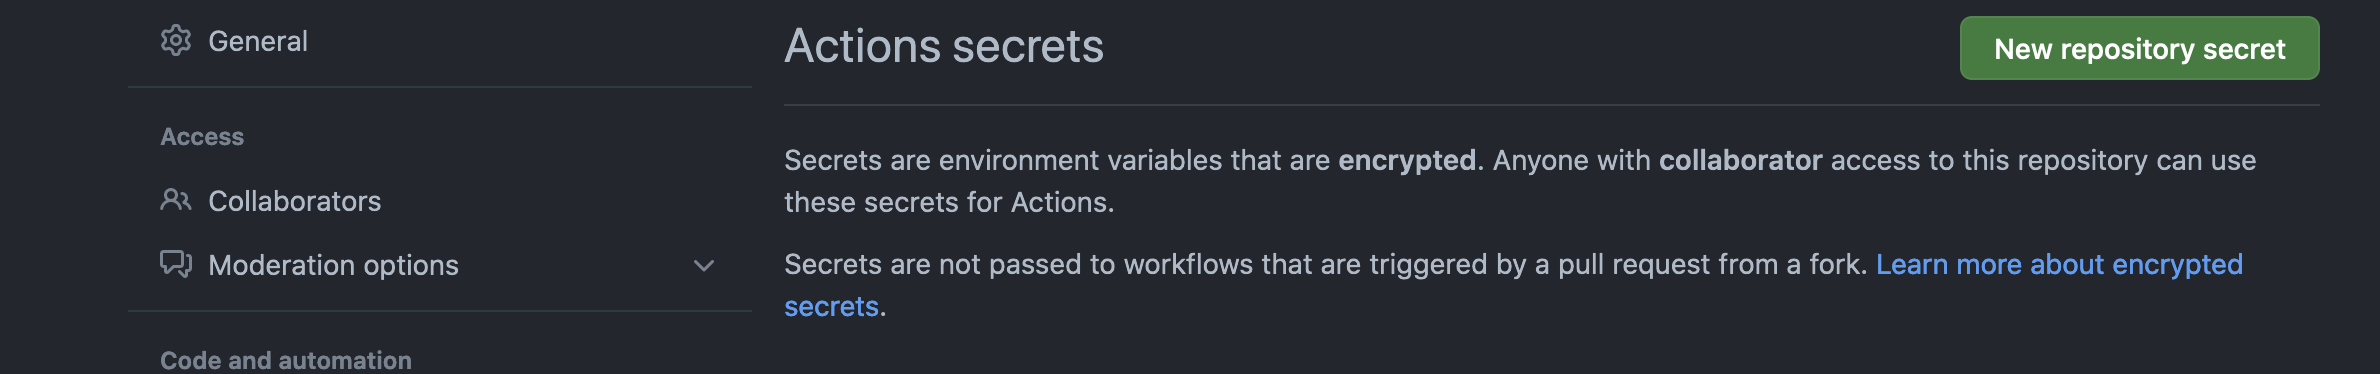
\includegraphics[width=8.cm, height=2cm]{generate_new_rep.png}
      \item Set the name \texttt{GH\_TOKEN} and paste the previous token generated.
      \item Now your token is stored and usable within this repository
      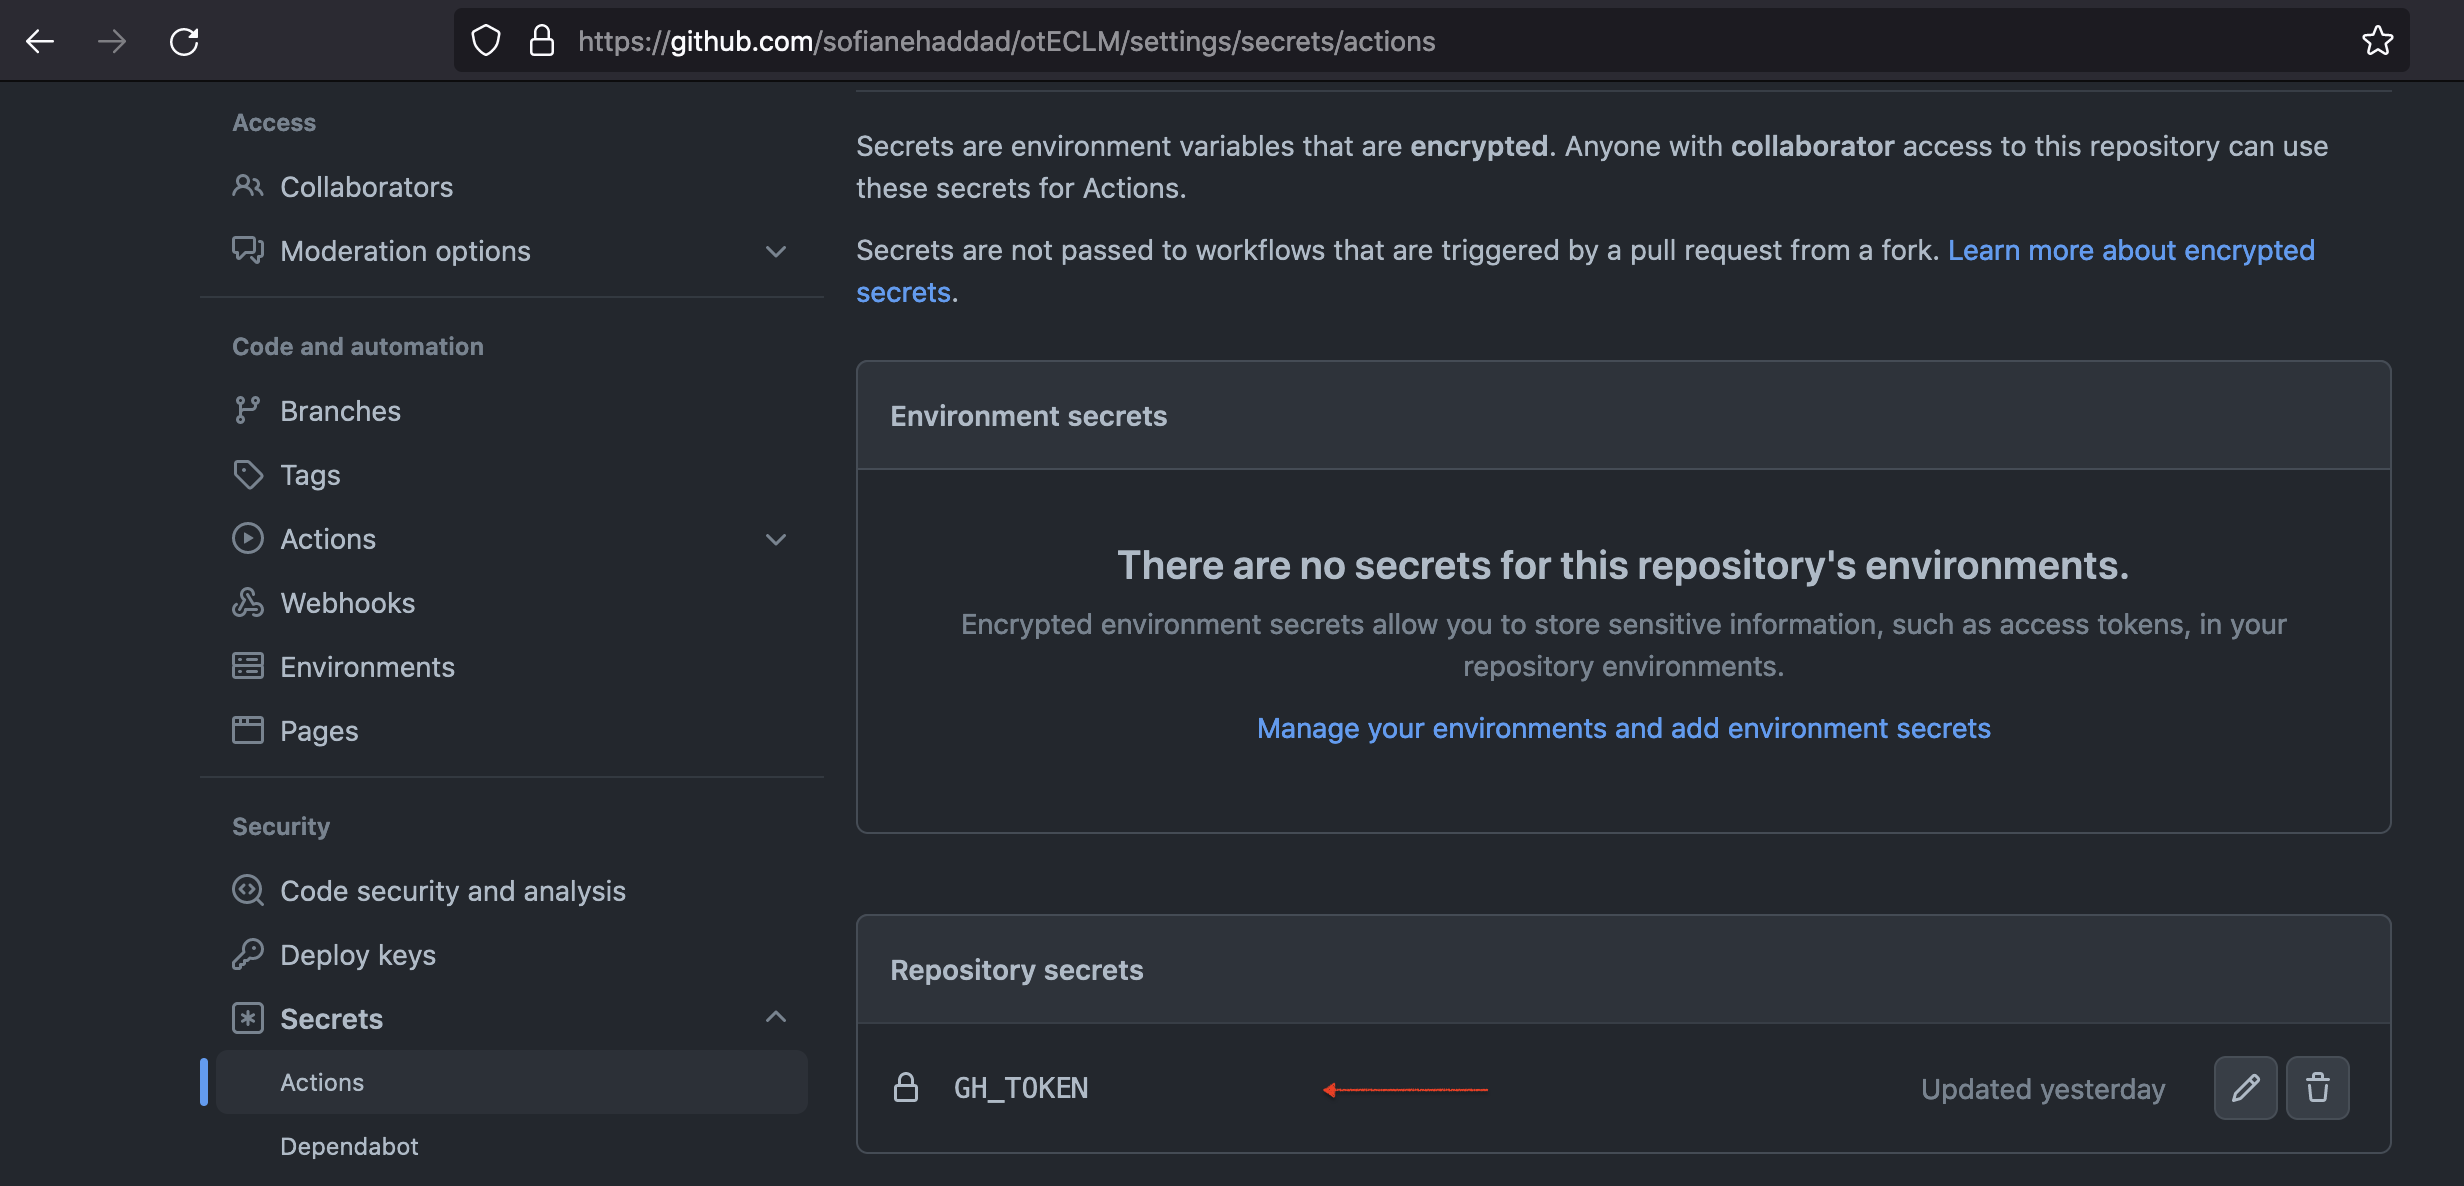
\includegraphics[width=8.cm, height=4cm]{refer_token.png}
      \end{itemize}
\end{frame}


\begin{frame}
  \frametitle{Module development: upload documentation using github and continuous integration}
  Finally we have all elements to deploy the documentation. To complete :
    \begin{itemize} 
      \item We should make sure to have a repository where upload is done (many often, \texttt{username.github.io}).\\
       This should contains an html index file. A minimal index could be provide.
       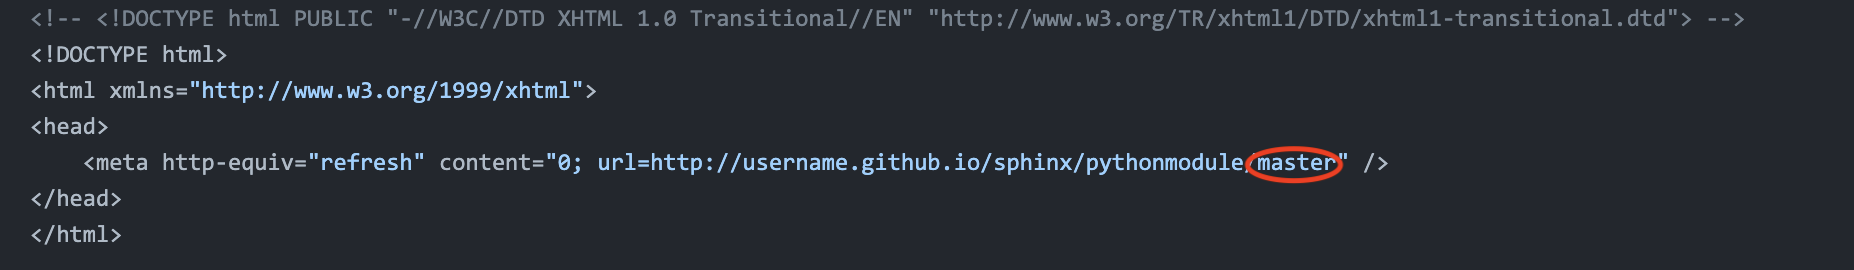
\includegraphics[width=9.cm]{index_minimal.png}
      \item Add corresponding instructions into continuous-integration script to upload on the previous repository
      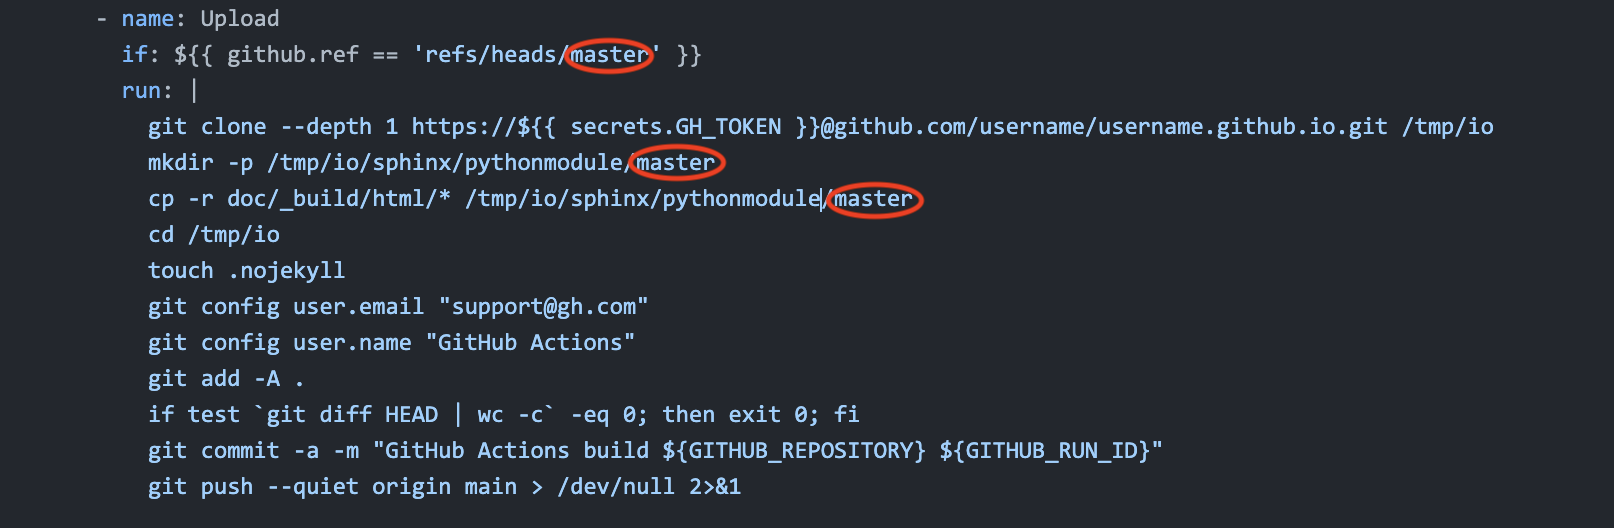
\includegraphics[width=9.cm]{instruction_ci.png}
    \end{itemize}
    Note: Keep in mind to replace \texttt{master} by \texttt{main} or other specific branch (release,...) with respect to the branch of interest.
\end{frame}

\end{document}
